\documentclass[nostrict]{szablonPG}

%-------------------- Dodatkowe pakiety ---------------------
\usepackage{listing_schemat}
%------------------------------------------------------------

%------------------------------------------------------------
%			      Pocz�tek pracy dyplomowej  
%------------------------------------------------------------

\begin{document}

%------------------------------------------------------------
%  Dodanie strony tytu�owej wygenerowanej z MojaPG oraz 
%  						o�wiadczenia

%\includepdf{meta/strona_tytulowa.pdf}
%\includepdf{meta/oswiadczenie.pdf}

%------------------------------------------------------------
%  Dodanie streszczenia i abstract
%  						

\chapter*{Streszczenie}
\indent Lorem Lorem ipsum dolor sit amet, consectetur adipiscing elit. Vivamus elementum arcu nec blandit aliquam. Integer eros dolor, molestie eget dictum quis, luctus sit amet sapien. Proin dignissim felis in ornare volutpat. Morbi vulputate rutrum efficitur. Ut vehicula vehicula metus, et iaculis tortor mattis vel. Nam blandit, arcu quis ultricies blandit, libero ante commodo augue, in accumsan dui leo at orci. Phasellus in augue et velit pulvinar malesuada ut et sem. Nulla vehicula nibh eu odio sollicitudin sagittis. Praesent condimentum semper neque, tincidunt luctus nisl scelerisque sed. Orci varius natoque penatibus et magnis dis parturient montes, nascetur ridiculus mus. 
\vspace{0.5cm}\newline
\textbf{S�owa kluczowe:} lorem ipsum, dolor sit amet, consectetur adipiscing\vspace{0.5cm}

\noindent \textbf{Dziedzina nauki i techniki, zgodnie z wymogami OECD:} nauki in�ynieryjne i techniczne, robotyka i automatyka

\chapter*{Abstract}
\indent This paper describe.... Lorem ipsum dolor sit amet, consectetur adipiscing elit. Vivamus elementum arcu nec blandit aliquam. Integer eros dolor, molestie eget dictum quis, luctus sit amet sapien. Proin dignissim felis in ornare volutpat. Morbi vulputate rutrum efficitur. Ut vehicula vehicula metus, et iaculis tortor mattis vel. Nam blandit, arcu quis ultricies blandit, libero ante commodo augue, in accumsan dui leo at orci. Phasellus in augue et velit pulvinar malesuada ut et sem. Nulla vehicula nibh eu odio sollicitudin sagittis. Praesent condimentum semper neque, tincidunt luctus nisl scelerisque sed. Orci varius natoque penatibus et magnis dis parturient montes, nascetur ridiculus mus. 
\vspace{0.5cm}\newline
\textbf{Keywords:} lorem ipsum, dolor sit amet, consectetur adipiscin \vspace{0.5cm}

%------------------------------------------------------------
%	Utworzenie spisu tre�ci pracy dyplomowej
\tableofcontents

%------------------------------------------------------------
%	Dodanie wykazu wazniejszych skr�t�w i oznacze� 
\chapter*{Wykaz wa�niejszych oznacze� i skr�t�w} % section* - ukrywa numerowanie oraz wyklucza ze spisu tresci
\addcontentsline{toc}{chapter}{Wykaz wa�niejszych oznacze� i skr�t�w}% % reczne dodanie do spisu tresci
\noindent EKG -- Elektrokardiografia\newline
HR -- T�tno (Heart Rate)\newline
HRV -- Zmienno�� rytmu serca (Heart Rate Variability)\newline
RSA -- Oddechowa arytmia zatokowa (Respiratory Sinus Arrhythmia)\newline
SDNN -- Odchylenie standardowe odst�p�w NN (Standard Deviation of NN intervals)\newline
RMSSD -- Pierwiastek kwadratowy z u�rednionych kwadrat�w r�nic kolejnych odst�p�w NN (Root Mean Square of Successive Differences)\newline
NN50 -- Liczba odst�p�w NN r�ni�cych si� o wi�cej ni� 50 ms (Number of NN intervals differing by more than 50 ms)\newline
pNN50 -- Proporcja odst�p�w NN50 do ca�kowitej liczby odst�p�w NN (Proportion of NN50 intervals to the total number of NN intervals)\newline
SDANN -- Odchylenie standardowe �rednich odst�p�w NN (Standard Deviation of the Averages of NN intervals)\newline
FFT -- Szybka transformacja Fouriera (Fast Fourier Transform)\newline
PSD -- Widmowa g�sto�� mocy (Power Spectral Density)\newline
FFTPSD -- Widmowa g�sto�� mocy oparta na szybkiej transformacji Fouriera (Fast Fourier Transform Power Spectral Density)\newline
ULF -- Ultra niskie cz�stotliwo�ci (Ultra Low Frequency)\newline
VLF -- Bardzo niskie cz�stotliwo�ci (Very Low Frequency)\newline
LF -- Niskie cz�stotliwo�ci (Low Frequency)\newline
HF -- Wysokie cz�stotliwo�ci (High Frequency)\newline
UHF -- Ultra wysokie cz�stotliwo�ci (Ultra High Frequency)\newline
SNR -- Stosunek sygna�u do szumu (Signal-to-noise Ratio)\newline
AF -- Migotanie przedsionk�w (Atrial Fibrillation)\newline
PPG -- Fotopletyzmografia (Photoplethysmography)\newline
DNN -- G��bokie sieci neuronowe (Deep Neural Network)\newline
LSTM -- Typ rekurencyjnej sieci neuronowej (Long Short-term Memory)\newline
CNN -- Splotowe sieci neuronowe (Convolutional Neural Network)\newline
SVM -- Maszyny wektor�w no�nych (Support Vector Machines)\newline
KNN -- Algorytm k-najbli�szych s�siad�w (K-Nearest Neighbours)\newline
API -- Interfejs programistyczny aplikacji (Application Programming Interface)\newline
SDK -- Zestaw narz�dzi programistycznych (Software Development Kit)\newline
BLE -- Bluetooth Low Energy\newline
MSE -- B��d �redniokwadratowy (Mean Squared Error)\newline
RMSE -- Pierwiastek z b��du �redniokwadratowego (Root Mean Squared Error)\newline
F1 -- Miara F-Score\newline
CWT -- Ci�g�a transformacja falkowa (Continuous Wavelet Transform)\newline
NREM -- Faza snu NREM (Non-rapid Eye Movement)\newline
REM -- Faza snu REM (Rapid Eye Movement)\newline

%------------------------------------------------------------
%	Dodanie rozdzia��w pracy dyplomowej - g��wne cia�o dokumentu 

\chapter{Wst�p i cel pracy} 
Lorem ipsum dolor sit amet, consectetur adipiscing elit. Vivamus elementum arcu nec blandit aliquam. Integer eros dolor, molestie eget dictum quis, luctus sit amet sapien. Proin dignissim felis in ornare volutpat. Morbi vulputate rutrum efficitur. Ut vehicula vehicula metus, et iaculis tortor mattis vel. Nam blandit, arcu quis ultricies blandit, libero ante commodo augue, in accumsan dui leo at orci. Phasellus in augue et velit pulvinar malesuada ut et sem. Nulla vehicula nibh eu odio sollicitudin sagittis. Praesent condimentum semper neque, tincidunt luctus nisl scelerisque sed. Orci varius natoque penatibus et magnis dis parturient montes, nascetur ridiculus mus.

Donec in libero a enim tempor finibus. Etiam in turpis sed metus ultricies pharetra vitae a ipsum. Nullam elementum est a vehicula convallis. Praesent vel eleifend quam, id eleifend tortor. Vestibulum non sollicitudin arcu. Nunc ultricies, ex sit amet faucibus elementum, erat est finibus lacus, non porttitor metus mi sed purus. Mauris at volutpat quam. Nam vel varius elit. Donec a urna vitae felis posuere facilisis. Suspendisse id enim quis massa imperdiet ultrices quis eu nibh. Pellentesque in elit ut tortor pharetra condimentum. Fusce non dapibus arcu, non blandit odio. Suspendisse faucibus fermentum neque quis dapibus.

Maecenas tincidunt est sit amet porttitor suscipit. Nullam rutrum lectus ut odio cursus facilisis. Donec fermentum, dolor sed sagittis congue, augue nisi sagittis nulla, nec ultricies sem elit non nibh. Vivamus erat ante, volutpat nec lectus in, finibus iaculis velit. Phasellus vel hendrerit dolor. Cras gravida ac lacus sit amet euismod. Integer venenatis ut tortor id tristique. Lorem ipsum dolor sit amet, consectetur adipiscing elit. Curabitur pellentesque ut ex ac volutpat. Suspendisse pellentesque tempus tempus. Nullam pharetra purus nunc, vitae eleifend ligula consectetur vel. Mauris quis quam non massa vestibulum lobortis. Donec suscipit tortor ut dictum vestibulum. Vestibulum ante ipsum primis in faucibus orci luctus et ultrices posuere cubilia Curae; Praesent ut finibus risus. Suspendisse sed risus ultricies, accumsan metus vitae, dignissim justo.

Vestibulum lorem elit, ornare vitae ultrices non, rhoncus eu elit. Vestibulum et gravida erat. Sed ut velit sollicitudin, blandit libero nec, maximus felis. Morbi feugiat pharetra lacus sit amet sodales. Aenean a sem elit. Ut et augue justo. Sed id consequat magna, non tincidunt eros. Sed congue tellus vitae ipsum commodo, nec pretium quam congue. Fusce non imperdiet sem, at imperdiet nibh. Morbi convallis nisl ante. Maecenas hendrerit, augue ac pretium molestie, ex massa lacinia est, sit amet volutpat eros magna vel erat.

Nunc egestas mauris sit amet sem facilisis, in rutrum quam faucibus. Etiam ornare fringilla tellus, sit amet bibendum nulla fermentum vitae. Nullam nec consectetur ipsum. Duis pulvinar libero vel diam lacinia, ac dapibus massa malesuada. Nullam sit amet gravida risus, nec tincidunt enim. Integer vehicula, nisl vitae hendrerit molestie, arcu arcu eleifend enim, at tempus odio leo nec nibh. Sed ut tortor risus. Nulla mattis pretium gravida. Phasellus eu augue magna. Proin quis dolor consectetur, accumsan velit et, maximus ipsum. 
\chapter{Drugi rozdzia�}
Lorem ipsum dolor sit amet, consectetur adipiscing elit. Vivamus elementum arcu nec blandit aliquam. Integer eros dolor, molestie eget dictum quis, luctus sit amet sapien. Proin dignissim felis in ornare volutpat. Morbi vulputate rutrum efficitur. Ut vehicula vehicula metus, et iaculis tortor mattis vel. Nam blandit, arcu quis ultricies blandit, libero ante commodo augue, in accumsan dui leo at orci. Phasellus in augue et velit pulvinar malesuada ut et sem. Nulla vehicula nibh eu odio sollicitudin sagittis. Praesent condimentum semper neque, tincidunt luctus nisl scelerisque sed. Orci varius natoque penatibus et magnis dis parturient montes, nascetur ridiculus mus.

Donec in libero a enim tempor finibus. Etiam in turpis sed metus ultricies pharetra vitae a ipsum. Nullam elementum est a vehicula convallis. Praesent vel eleifend quam, id eleifend tortor. Vestibulum non sollicitudin arcu. Nunc ultricies, ex sit amet faucibus elementum, erat est finibus lacus, non porttitor metus mi sed purus. Mauris at volutpat quam. Nam vel varius elit. Donec a urna vitae felis posuere facilisis. Suspendisse id enim quis massa imperdiet ultrices quis eu nibh. Pellentesque in elit ut tortor pharetra condimentum. Fusce non dapibus arcu, non blandit odio. Suspendisse faucibus fermentum neque quis dapibus.
\section{Pierwsza sekcja}
Maecenas tincidunt est sit amet porttitor suscipit. Nullam rutrum lectus ut odio cursus facilisis. Donec fermentum, dolor sed sagittis congue, augue nisi sagittis nulla, nec ultricies sem elit non nibh. Vivamus erat ante, volutpat nec lectus in, finibus iaculis velit. Phasellus vel hendrerit dolor. Cras gravida ac lacus sit amet euismod. Integer venenatis ut tortor id tristique. Lorem ipsum dolor sit amet, consectetur adipiscing elit. Curabitur pellentesque ut ex ac volutpat. Suspendisse pellentesque tempus tempus. Nullam pharetra purus nunc, vitae eleifend ligula consectetur vel. Mauris quis quam non massa vestibulum lobortis. Donec suscipit tortor ut dictum vestibulum. Vestibulum ante ipsum primis in faucibus orci luctus et ultrices posuere cubilia Curae; Praesent ut finibus risus. Suspendisse sed risus ultricies, accumsan metus vitae, dignissim justo.
\subsection{Pierwsza podsekcja}

\begin{figure}[ht]
\centering
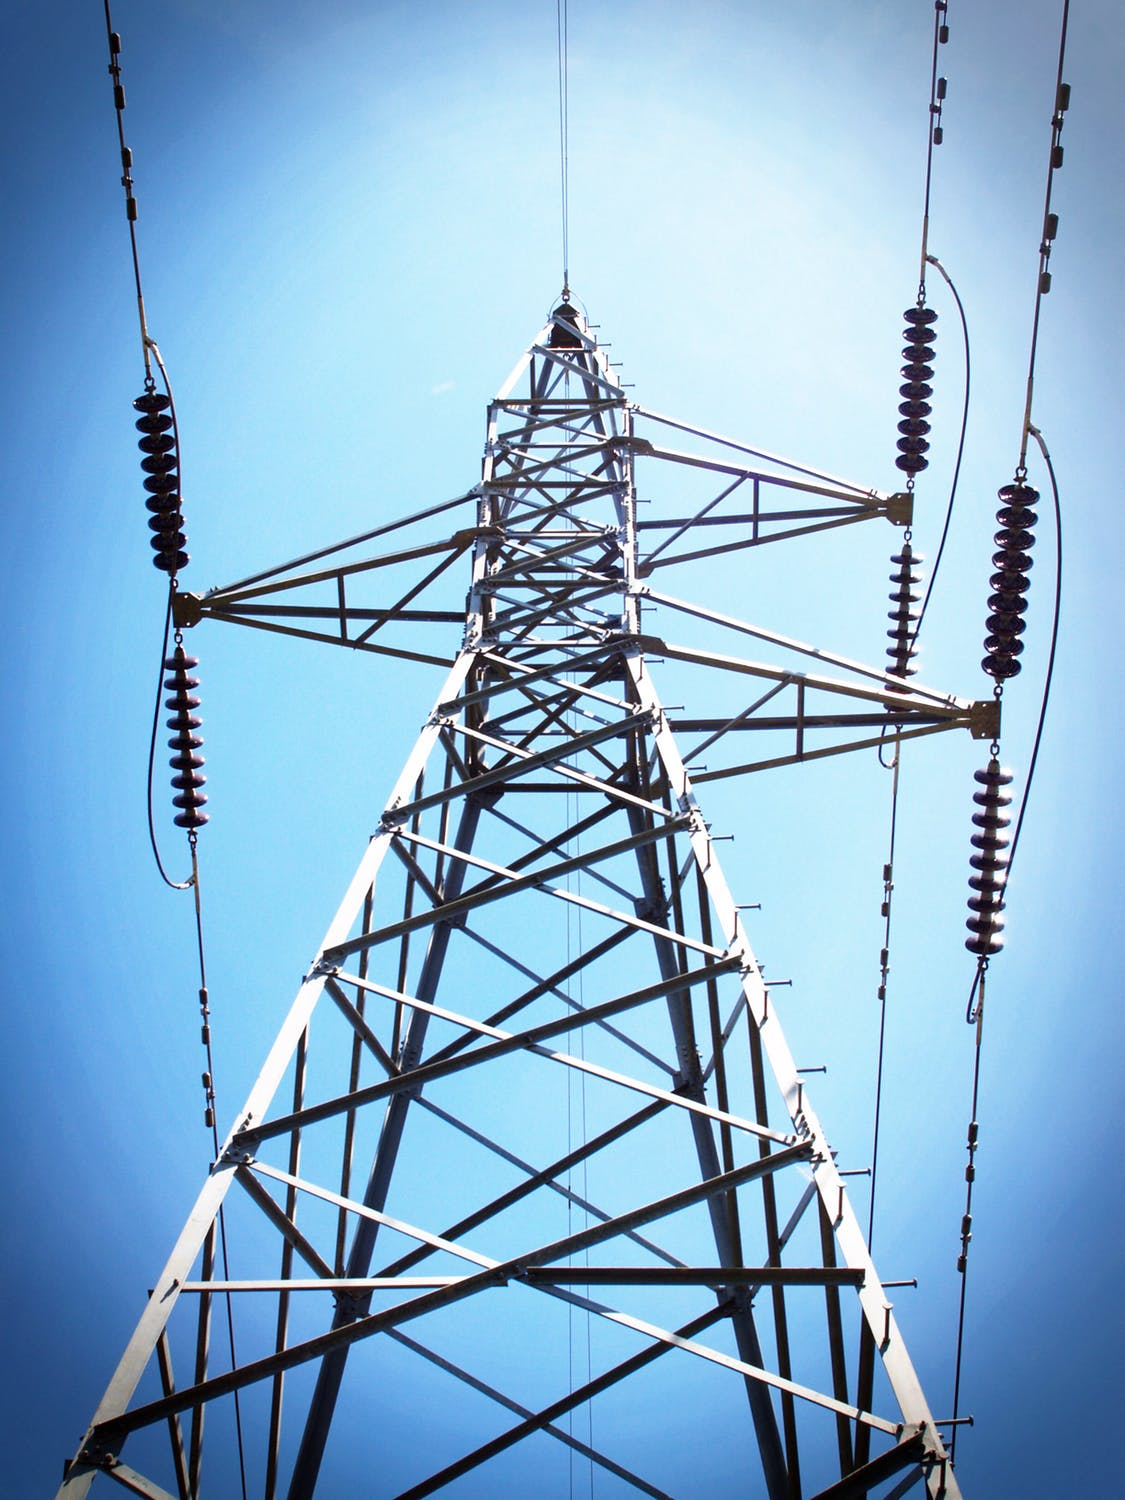
\includegraphics[scale=0.25]{rysunki/example}
\caption{Przyk�adowy obraz zamieszczony w pracy dyplomowej}
\label{img/template1}
\end{figure}
Vestibulum lorem elit, ornare vitae ultrices non, rhoncus eu elit. Vestibulum et gravida erat. Sed ut velit sollicitudin, blandit libero nec, maximus felis. Morbi feugiat pharetra lacus sit amet sodales. Aenean a sem elit. Ut et augue justo. Sed id consequat magna, non tincidunt eros. Sed congue tellus vitae ipsum commodo, nec pretium quam congue. Fusce non imperdiet sem, at imperdiet nibh. Morbi convallis nisl ante. Maecenas hendrerit, augue ac pretium molestie, ex massa lacinia est, sit amet volutpat eros magna vel erat.

Nunc egestas mauris sit amet sem facilisis, in rutrum quam faucibus. Etiam ornare fringilla tellus, sit amet bibendum nulla fermentum vitae. Nullam nec consectetur ipsum. Duis pulvinar libero vel diam lacinia, ac dapibus massa malesuada. Nullam sit amet gravida risus, nec tincidunt enim. Integer vehicula, nisl vitae hendrerit molestie, arcu arcu eleifend enim, at tempus odio leo nec nibh. Sed ut tortor risus. Nulla mattis pretium gravida. Phasellus eu augue magna. Proin quis dolor consectetur, accumsan velit et, maximus ipsum. 

Vestibulum lorem elit, ornare vitae ultrices non, rhoncus eu elit. Vestibulum et gravida erat. Sed ut velit sollicitudin, blandit libero nec, maximus felis. Morbi feugiat pharetra lacus sit amet sodales. Aenean a sem elit. Ut et augue justo. Sed id consequat magna, non tincidunt eros. Sed congue tellus vitae ipsum commodo, nec pretium quam congue. Fusce non imperdiet sem, at imperdiet nibh. Morbi convallis nisl ante. Maecenas hendrerit, augue ac pretium molestie, ex massa lacinia est, sit amet volutpat eros magna vel erat.

\begin{table}[ht]
\captionsetup{justification=centering}
\caption{Dane techniczne silnika nap�dowego uk�adu jezdnego}
\centering
    \begin{tabular}{|l|l|c|}
    \hline
    \multicolumn{1}{|l|}{\textbf{Lp.}} & \multicolumn{1}{l|}{\textbf{Parametr}} & \multicolumn{1}{c|}{\textbf{Warto��}} \\
    \hline
       1.   & Napi�cie zasilania [V] & 12  \\
    \hline
       2.   &  Pr�dko�� obrotowa [obr/min]& 200\\
    \hline
       3.  & Moment obrotowy [Nm]   & 0.8 \\
    \hline
       4.  & Maks. pr�d pracy [A]      &  0.8 \\
    \hline
       5.  & �rednica wa�u [mm]     &  8 \\
    \hline
       6.  & Rodzaj czujnika     &  Inkrementalny   \\
    \hline
       7.  & Rozdzielczo�� enkodera [imp/obr]   &  75 \\
    \hline
    \end{tabular}
  \label{silnik_skret}
\end{table}

Nunc egestas mauris sit amet sem facilisis, in rutrum quam faucibus. Etiam ornare fringilla tellus, sit amet bibendum nulla fermentum vitae. Nullam nec consectetur ipsum. Duis pulvinar libero vel diam lacinia, ac dapibus massa malesuada. Nullam sit amet gravida risus, nec tincidunt enim. Integer vehicula, nisl vitae hendrerit molestie, arcu arcu eleifend enim, at tempus odio leo nec nibh. Sed ut tortor risus. Nulla mattis pretium gravida. Phasellus eu augue magna. Proin quis dolor consectetur, accumsan velit et, maximus ipsum. 



Nunc egestas mauris sit amet sem facilisis, in rutrum quam faucibus. Etiam ornare fringilla tellus, sit amet bibendum nulla fermentum vitae. Nullam nec consectetur ipsum. Duis pulvinar libero vel diam lacinia, ac dapibus massa malesuada. Nullam sit amet gravida risus, nec tincidunt enim. Integer vehicula, nisl vitae hendrerit molestie, arcu arcu eleifend enim, at tempus odio leo nec nibh. Sed ut tortor risus. Nulla mattis pretium gravida. Phasellus eu augue magna. Proin quis dolor consectetur, accumsan velit et, maximus ipsum. 


Nunc egestas mauris sit amet sem facilisis, in rutrum quam faucibus. Etiam ornare fringilla tellus, sit amet bibendum nulla fermentum vitae. Nullam nec consectetur ipsum. Duis pulvinar libero vel diam lacinia, ac dapibus massa malesuada. Nullam sit amet gravida risus, nec tincidunt enim. Integer vehicula, nisl vitae hendrerit molestie, arcu arcu eleifend enim, at tempus odio leo nec nibh. Sed ut tortor risus. Nulla mattis pretium gravida. Phasellus eu augue magna. Proin quis dolor consectetur, accumsan velit et, maximus ipsum. 

\begin{equation}
\label{rownanie}
\sum_{n=1}^{\infty} 2^{-n} \arccos(\frac{\int_{a}^{b} x^2 dx}{x})  = 1
\end{equation}

Nunc egestas mauris sit amet sem facilisis, in rutrum quam faucibus. Etiam ornare fringilla tellus, sit amet bibendum nulla fermentum vitae. Nullam nec consectetur ipsum. Duis pulvinar libero vel diam lacinia, ac dapibus massa malesuada. Nullam sit amet gravida risus, nec tincidunt enim. Integer vehicula, nisl vitae hendrerit molestie, arcu arcu eleifend enim, at tempus odio leo nec nibh. Sed ut tortor risus. Nulla mattis pretium gravida. Phasellus eu augue magna. Proin quis dolor consectetur, accumsan velit et, maximus ipsum. 

\lstset{style=matlab}

\begin{lstlisting}[caption={Przyk�adowy listing programu Matlab}]
for n = 1 : 4
    
    for j = 1 : 100
        Imp_1_100(n,j) = (R1*R2*C2*i*j*2*pi + R1 + R2);
    end
    
    % Zmiana warto�ci  
    
    if log(abs(Imp_1_100(n,100))) - log(Rr) <= 2
        Rr = Rr/10;
    end
    
    RT(n) = Rr;  % Przypisanie warto�ci
end
\end{lstlisting}


\lstset{style=java}

\begin{lstlisting}[caption={Przyk�adowy listing w j�zyku Java},label=javovy]
class OuterClass {
  int x = 10;

  private class InnerClass {
    int y = 5;
  }
}

public class MyMainClass {
  public static void main(String[] args) {
    OuterClass myOuter = new OuterClass();
    OuterClass.InnerClass myInner = myOuter.new InnerClass();
    System.out.println(myInner.y + myOuter.x);
  }
}
\end{lstlisting}

\newpage





\lstset{style=vhdl}

\begin{lstlisting}[caption={Przyk�adowy listing w j�zyku VHDL}]

architecture FSMD of gcd is
begin

    process(rst, clk)

    -- define states using variable 
    type S_Type is (ST0, ST1, ST2);
    variable State: S_Type := ST0 ;			
    variable Data_X, Data_Y: unsigned(3 downto 0);
	
    begin

        if (rst='1') then		    -- initialization
	    d_o <= "0000";
	    State := ST0;
	elsif (clk'event and clk='1') then
	    case State is
	        when ST0 =>		    -- starting
		    if (go_i='1') then
			Data_X := x_i;
			Data_Y := y_i;
			State := ST1;
		    else
		        State := ST0;
		    end if;
		when ST1 =>		    -- idle state 
		    State := ST2;
		when ST2 =>		    -- computation
		    if (Data_X/=Data_Y) then
		        if (Data_X<Data_Y) then
			    Data_Y := Data_Y - Data_X;
			else
			    Data_X := Data_X - Data_Y;
			end if;
			State := ST1;
		    else
			d_o <=Data_X;       -- done
		        State := ST0;
		    end if;
		when others =>		    -- go back 
		    d_o <= "ZZZZ";
		    State := ST0;
            end case;				
 	end if;
    
    end process;		

end FSMD;

\end{lstlisting}


Nunc egestas mauris sit amet sem facilisis, in rutrum quam faucibus. Etiam ornare fringilla tellus, sit amet bibendum nulla fermentum vitae. Nullam nec consectetur ipsum. Duis pulvinar libero vel diam lacinia, ac dapibus massa malesuada. Nullam sit amet gravida risus, nec tincidunt enim. Integer vehicula, nisl vitae hendrerit molestie, arcu arcu eleifend enim, at tempus odio leo nec nibh. Sed ut tortor risus. Nulla mattis pretium gravida. Phasellus eu augue magna. Proin quis dolor consectetur, accumsan velit et, maximus ipsum. 
Nunc egestas mauris sit amet sem facilisis, in rutrum quam faucibus. Etiam ornare fringilla tellus, sit amet bibendum nulla fermentum vitae. Nullam nec consectetur ipsum. Duis pulvinar libero vel diam lacinia, ac dapibus massa malesuada. Nullam sit amet gravida risus, nec tincidunt enim. Integer vehicula, nisl vitae hendrerit molestie, arcu arcu eleifend enim, at tempus odio leo nec nibh. Sed ut tortor risus. Nulla mattis pretium gravida. Phasellus eu augue magna. Proin quis dolor consectetur, accumsan velit et, maximus ipsum. 

Nunc egestas mauris sit amet sem facilisis, in rutrum quam faucibus. Etiam ornare fringilla tellus, sit amet bibendum nulla fermentum vitae. Nullam nec consectetur ipsum. Duis pulvinar libero vel diam lacinia, ac dapibus massa malesuada. Nullam sit amet gravida risus, nec tincidunt enim. Integer vehicula, nisl vitae hendrerit molestie, arcu arcu eleifend enim, at tempus odio leo nec nibh. Sed ut tortor risus. Nulla mattis pretium gravida. Phasellus eu augue magna. Proin quis dolor consectetur, accumsan velit et, maximus ipsum. 



% Definition of blocks:
\tikzset{%
  block/.style    = {draw, thick, rectangle, minimum height = 3em,
    minimum width = 3em},
  sum/.style      = {draw, circle, node distance = 2cm}, % Adder
  input/.style    = {coordinate}, % Input
  output/.style   = {coordinate} % Output
}
% Defining string as labels of certain blocks.
\newcommand{\suma}{\Large$+$}
\newcommand{\inte}{$\displaystyle \int$}
\newcommand{\derv}{\huge$\frac{d}{dt}$}

\begin{figure}[ht]

\begin{tikzpicture}[auto, thick, node distance=2cm, >=triangle 45]
\draw
	% Drawing the blocks of first filter :
	node at (0,0)[right=-3mm]{\Large }
	node [input, name=input1] {} 
	node [sum, right of=input1] (suma1) {\suma}
	node [block, right of=suma1] (inte1) {\inte}
         node at (6.8,0)[block] (Q1) {\Large $Q_1$}
         node [block, below of=inte1] (ret1) {\Large$T_1$$$};
    % Joining blocks. 
    % Commands \draw with options like [->] must be written individually
	\draw[->](input1) -- node {$X(Z)$}(suma1);
 	\draw[->](suma1) -- node {} (inte1);
	\draw[->](inte1) -- node {} (Q1);
	\draw[->](ret1) -| node[near end]{} (suma1);
	% Adder
\draw
	node at (5.4,-4) [sum, name=suma2] {\suma}
    	% Second stage of filter 
	node at  (1,-6) [sum, name=suma3] {\suma}
	node [block, right of=suma3] (inte2) {\inte}
	node [sum, right of=inte2] (suma4) {\suma}
	node [block, right of=suma4] (inte3) {\inte}
	node [block, right of=inte3] (Q2) {\Large$Q_2$$$}
	node at (9,-8) [block, name=ret2] {\Large$T_2$$$}
;
	% Joining the blocks of second filter
	\draw[->] (suma3) -- node {} (inte2);
	\draw[->] (inte2) -- node {} (suma4);
	\draw[->] (suma4) -- node {} (inte3);
	\draw[->] (inte3) -- node {} (Q2);
	\draw[->] (ret2) -| (suma3);
	\draw[->] (ret2) -| (suma4);
         % Third stage of filter:
	% Defining nodes:
\draw
	node at (11.5, 0) [sum, name=suma5]{\suma}
	node [output, right of=suma5]{}
	node [block, below of=suma5] (deriv1){\derv}
	node [output, right of=suma5] (sal2){}
;
	% Joining the blocks:
	\draw[->] (suma2) -| node {}(suma3);
	\draw[->] (Q1) -- (8,0) |- node {}(ret1);
	\draw[->] (8,0) |- (suma2);
	\draw[->] (5.4,0) -- (suma2);
	\draw[->] (Q1) -- node {}(suma5);
	\draw[->] (deriv1) -- node {}(suma5);
	\draw[->] (Q2) -| node {}(deriv1);
    	\draw[<->] (ret2) -| node {}(deriv1);
    	\draw[->] (suma5) -- node {$Y(Z)$}(sal2);
    	% Drawing nodes with \textbullet
\draw
	node at (8,0) {\textbullet} 
	node at (8,-2){\textbullet}
	node at (5.4,0){\textbullet}
    	node at (5,-8){\textbullet}
    	node at (11.5,-6){\textbullet}
    	;
	% Boxing and labelling noise shapers
	\draw [color=gray,thick](-0.5,-3) rectangle (9,1);
	\node at (-0.5,1) [above=5mm, right=0mm] {\textsc{generator szumu I rz�du}};
	\draw [color=gray,thick](-0.5,-9) rectangle (12.5,-5);
	\node at (-0.5,-9) [below=5mm, right=0mm] {\textsc{generator szumu II rz�du}};
\end{tikzpicture}
\caption{Przyk�adowy schemat blokowy utworzony przy u�yciu pakietu tikz}
\end{figure}

Nunc egestas mauris sit amet sem facilisis, in rutrum quam faucibus. Etiam ornare fringilla tellus, sit amet bibendum nulla fermentum vitae. Nullam nec consectetur ipsum. Duis pulvinar libero vel diam lacinia, ac dapibus massa nc egestas mauris sit amet sem facilisis, in rutrum quam faucibus. Etiam ornare fringilla tellus, sit amet bibendum nulla fermentum vitae. Nullam nec consectetur ipsum. Duis pulvinar libero vel diam lacinia, ac dapibus massa.




%\input{rozdzialy/przyklad_rozdzialu_3.tex}

% itd...

% ---------------------- Bibliografia -----------------------
\bibliographystyle{plain}
\begin{thebibliography}{99}
    \addcontentsline{toc}{chapter}{Wykaz literatury}
    \small

    %------------------------------------------
    %Lilly, Leonard S. (2016). Pathophysiology of Heart Disease: A Collaborative Project of Medical Students and Faculty, 6th Edition. Lippincott Williams & Wilkins. pp. 70�78. ISBN 978-1-4698-9758-5. OCLC 1229852550.

    \bibitem{Lilly-Pathophysiology}
    Leonard S. Lilly \emph{Pathophysiology of Heart Disease: A Collaborative Project of Medical Students and Faculty, 6th Edition.} Lippincott Williams \& Wilkins. pp. 70�78. ISBN 978-1-4698-9758-5. OCLC 1229852550.
    %------------------------------------------

    %------------------------------------------
    \bibitem{Malik-HRV}
    Task Force of the European Society of Cardiology, \& North American Society of Pacing and Electrophysiology \emph{Heart rate variability: Standards of measurement, physiological interpretation, and clinical use.} In: Circulation. 1996, pp. 1043-1065. doi:10.1161/01.CIR.93.5.1043.
    %PDF
    %https://www.ahajournals.org/doi/10.1161/01.CIR.93.5.1043
    %https://www.researchgate.net/publication/279548912_Heart_rate_variability_Standards_of_measurement_physiological_interpretation_and_clinical_use
    %------------------------------------------

    %------------------------------------------
    \bibitem{Fariha-PanTompkins}
    M. A. Z. Fariha et al. \emph{Analysis of Pan-Tompkins Algorithm Performance with Noisy ECG Signals}, J. Phys.: Conf. Ser., vol. 1532, p. 012022, 2020. Available at: \href{https://iopscience.iop.org/article/10.1088/1742-6596/1532/1/012022/pdf}{https://iopscience.iop.org/article/10.1088/1742-6596/1532/1/012022/pdf.} [Accessed 08.11.2024]
    %https://iopscience.iop.org/article/10.1088/1742-6596/1532/1/012022/pdf}{https://iopscience.iop.org/article/10.1088/1742-6596/1532/1/012022/pdf
    %------------------------------------------

    %TO DO: dopasowa� strony glownie rozdzial 2
    \bibitem{Romano-ECG}
    M. Roman{\`o} and R. Bertona. \emph{Text Atlas of Practical Electrocardiography: A Basic Guide to ECG Interpretation.} Springer Milan, 2015. ISBN: 9788847057418. %Available at: \href{https://books.google.pl/books?id=qH8QBwAAQBAJ}{https://books.google.pl/books?id=qH8QBwAAQBAJ}. [Accessed 12.11.2024]

    % https://books.google.pl/books?hl=pl&lr=&id=qH8QBwAAQBAJ&oi=fnd&pg=PP17&dq=The+Practical+Guide+to+ECG+Interpretation&ots=xtUWsyms0z&sig=GFw3_NCeNPsIWaDzl1LhZNcJ4pY&redir_esc=y#v=onepage&q=The%20Practical%20Guide%20to%20ECG%20Interpretation&f=false
    %https://books.google.pl/books?id=qH8QBwAAQBAJ&printsec=frontcover&hl=pl&source=gbs_atb#v=onepage&q&f=false

    \bibitem{Goodfellow-DeepLearning}
    I. Goodfellow, Y. Bengio, and A. Courville, \emph{Deep Learning}. Cambridge, MA, USA: MIT Press, 2016. [Online]. Available: \url{http://www.deeplearningbook.org}[Accessed 25.11.2024]

    %------------------------------------------
    \bibitem{Bartsch-PhaseTransitions}
    R. P. Bartsch, A. Y. Schumann, J. W. Kantelhardt, T. Penzel, and P. Ch. Ivanov,
    \emph{Phase transitions in physiologic coupling},
    Proc. Natl. Acad. Sci. U. S. A., vol. 109, no. 26, pp. 10181�10186, Jun. 2012.
    Available at: \href{https://doi.org/10.1073/pnas.1204568109}{https://doi.org/10.1073/pnas.1204568109}. [Accessed 08.11.2024]
    %------------------------------------------

    \bibitem{MUzairZahid-UNET}
    M. U. Zahid, S. Kiranyaz, T. Ince, O. C. Devecioglu, M. E. H. Chowdhury, A. Khandakar, A. Tahir, and M. Gabbouj,
    \emph{Robust R-Peak Detection in Low-Quality Holter ECGs Using 1D Convolutional Neural Network},
    *IEEE Transactions on Biomedical Engineering*, vol. 69, no. 1, pp. 119--128, Jan. 2021.

    \bibitem{FDA_KardiaAI_2018}
    U.S. Food and Drug Administration, \emph{Kardia AI Clearance - K181823}, 2018. [Online]. Available: \url{https://www.accessdata.fda.gov/cdrh_docs/pdf18/K181823.pdf}. [Accessed: Dec. 1, 2024].

    % Bumgarner, J. M., Lambert, C. T., Hussein, A. A., et al. (2018). Smartwatch Algorithm for Automated Detection of Atrial Fibrillation. Journal of the American College of Cardiology, 71(21), 2381-2388. DOI: 10.1016/j.jacc.2018.03.003.
    \bibitem{Bumgarner2018}
    J.~M. Bumgarner, C.~T. Lambert, A.~A. Hussein, \textit{et al.}, ``Smartwatch Algorithm for Automated Detection of Atrial Fibrillation,'' \textit{Journal of the American College of Cardiology}, vol. 71, no. 21, pp. 2381--2388, 2018, doi: \url{10.1016/j.jacc.2018.03.003}.

    % https://pmc.ncbi.nlm.nih.gov/articles/PMC9971999/
    \bibitem{Raghunath2023}
    A. Raghunath, D.~D. Nguyen, M. Schram, D. Albert, S. Gollakota, L. Shapiro, and A.~R. Sridhar, ``Artificial intelligence-enabled mobile electrocardiograms for event prediction in paroxysmal atrial fibrillation,'' \textit{Cardiovascular Digital Health Journal}, vol. 4, no. 1, pp. 21--28, Jan. 2023, doi: \url{10.1016/j.cvdhj.2023.01.002}. PMID: 36865584; PMCID: PMC9971999.

    \bibitem{ribeiro2020automatic}
    Ribeiro, A.H., Ribeiro, M.H., Paix?o, G.M.M. \emph{et al.}, \emph{Automatic diagnosis of the 12-lead ECG using a deep neural network}, \emph{Nature Communications}, vol. 11, p. 1760, 2020, doi: 10.1038/s41467-020-15432-4.
    % Ribeiro, A.H., Ribeiro, M.H., Paix?o, G.M.M. et al. Automatic diagnosis of the 12-lead ECG using a deep neural network. Nat Commun 11, 1760 (2020). https://doi.org/10.1038/s41467-020-15432-4

    \bibitem{NAROTAMO-deepLearning}
    Deep learning for ECG classification: A comparative study of 1D and 2D representations and multimodal fusion approaches
    %     @article{NAROTAMO2024106141,
    % title = {Deep learning for ECG classification: A comparative study of 1D and 2D representations and multimodal fusion approaches},
    % journal = {Biomedical Signal Processing and Control},
    % volume = {93},
    % pages = {106141},
    % year = {2024},
    % issn = {1746-8094},
    % doi = {https://doi.org/10.1016/j.bspc.2024.106141},
    % url = {https://www.sciencedirect.com/science/article/pii/S174680942400199X},
    % author = {Hemaxi Narotamo and Mariana Dias and Ricardo Santos and Andr� V. Carreiro and Hugo Gamboa and Margarida Silveira},
    % keywords = {Electrocardiogram classification, Cardiovascular diseases, Deep learning, Recurrent neural networks, Convolutional neural networks, Multimodal artificial intelligence},
    % abstract = {The improved diagnosis of cardiovascular diseases (CVD) from electrocardiograms (ECG) may help prevent their severity. Since Deep Learning (DL) became popular, several DL methods have been developed for ECG classification. In this work, we compare how different methods for ECG signal representation perform in the multi-label classification of CVDs, including recent attention-based strategies. Furthermore, multimodal fusion strategies are employed to improve the prediction capacity of individual representation networks. The publicly available PTB-XL ECG dataset, which contains 21,837 records and labels for the diagnosis of 4 CVDs, was used for the task. Two DL strategies using different processing approaches were compared. Recurrent Neural Network-based models take advantage of the temporal dependence between raw signal values, namely through Gated Recurrent Unit (GRU), Long Short Term Memory (LSTM) and 1D-Convolutional Neural Network models. Additionally, the raw ECG was converted into image representations, based on recent work, and the classification was performed using distinct 2D-Convolutional Neural Networks. The potential of multimodal DL was then studied through early, late and joint data fusion strategies, to evaluate the benefit of resorting to multiple representations. Results based on the 1D ECG representation outperform image-based approaches and multimodal models. The best model, GRU, achieved sensitivity and specificity of 79.67% and 81.04%, respectively.}
    % }

    \bibitem{Morteza-RandomForest}
    Morteza Zabihi1*
    , Ali Bahrami Rad2*
    , Aggelos K. Katsaggelos3
    ,
    Serkan Kiranyaz4
    , Susanna Narkilahti2
    , and Moncef Gabbouj Detection of Atrial Fibrillation in ECG Hand-held Devices Using a Random
    Forest Classifier
    % https://physionet.org/files/challenge-2017/1.0.0/papers/069-336.pdf

    \bibitem{Bachmann-electrolyte_prediction}
    von Bachmann, P., Gedon, D., Gustafsson, F.K. et al. \emph{Evaluating regression and probabilistic methods for ECG-based electrolyte prediction.} Sci Rep 14, 15273 (2024). https://doi.org/10.1038/s41598-024-65223-w
    % von Bachmann, P., Gedon, D., Gustafsson, F.K. et al. Evaluating regression and probabilistic methods for ECG-based electrolyte prediction. Sci Rep 14, 15273 (2024). https://doi.org/10.1038/s41598-024-65223-w

    \bibitem{JUHO-LSTM}
    Laitala J., Jiang M., Haulivuori E., Kasaeyan Naeini E., Airola A., Rahmani A. M., Dutt N., Liljeberg P.:
    Robust ECG R-peak detection using LSTM, 2020, doi: 10.1145/3341105.3373945.
    %https://dl.acm.org/doi/pdf/10.1145/3341105.3373945

    \bibitem{PhysioNet-Challange2017}
    Clifford GD, Liu C, Moody B, Li-wei HL, Silva I, Li Q, Johnson AE, Mark RG. AF classification from a short single lead ECG recording: The PhysioNet/computing in cardiology challenge 2017. In 2017 Computing in Cardiology (CinC) 2017 Sep 24 (pp. 1-4). IEEE. https://doi.org/10.22489/CinC.2017.065-469

    \bibitem{Kavya-shockableArthytmiaDetection}
    Lakkakula Kavya, Karuna Yepuganti, Saladi Saritha, Allam Jaya Prakash, Kiran Kumar Patro, Suraj Prakash Sahoo, Ryszard Tadeusiewicz, Pawel Plawiak:
    A review of shockable arrhythmia detection of ECG signals using machine and deep learning techniques. Int. J. Appl. Math. Comput. Sci. 34
    % https://sciendo.com/article/10.61822/amcs-2024-0034


    \bibitem{Irungu-EcgCovid}
    J. Irungu, T. Oladunni, A. C. Grizzle, M. Denis, M. Savadkoohi, and E. Ososanya, "ML-ECG-COVID: A Machine Learning-Electrocardiogram Signal Processing Technique for COVID-19 Predictive Modeling," \textit{IEEE Access}, vol. 11, pp. 135994--136014, 2023, doi: 10.1109/ACCESS.2023.3335384.


%     @ARTICLE{10325461,
%   author={Irungu, John and Oladunni, Timothy and Grizzle, Andrew C. and Denis, Max and Savadkoohi, Marzieh and Ososanya, Esther},
%   journal={IEEE Access}, 
%   title={ML-ECG-COVID: A Machine Learning-Electrocardiogram Signal Processing Technique for COVID-19 Predictive Modeling}, 
%   year={2023},
%   volume={11},
%   number={},
%   pages={135994-136014},
%   keywords={Electrocardiography;Feature extraction;Support vector machines;Machine learning;Classification algorithms;Time-frequency analysis;Random forests;Nearest neighbor methods;Support vector machine (SVM);random forest;QRS complex;K-nearest neighbor (KNN);electrocardiogram (ECG)},
%   doi={10.1109/ACCESS.2023.3335384}}




    \bibitem{SAKR2023324}
    A.~S.~Sakr, P.~P�awiak, R.~Tadeusiewicz, J.~P�awiak, M.~Sakr, and M.~Hammad, "ECG-COVID: An end-to-end deep model based on electrocardiogram for COVID-19 detection," *Information Sciences*, vol. 619, pp. 324�339, 2023, doi: https://doi.org/10.1016/j.ins.2022.11.069

    %     @article{SAKR2023324,
    % title = {ECG-COVID: An end-to-end deep model based on electrocardiogram for COVID-19 detection},
    % journal = {Information Sciences},
    % volume = {619},
    % pages = {324-339},
    % year = {2023},
    % issn = {0020-0255},
    % doi = {https://doi.org/10.1016/j.ins.2022.11.069},
    % url = {https://www.sciencedirect.com/science/article/pii/S0020025522013585},
    % author = {Ahmed S. Sakr and Pawe� P�awiak and Ryszard Tadeusiewicz and Joanna P�awiak and Mohamed Sakr and Mohamed Hammad},
    % keywords = {COVID-19, ECG, CNN, End-to-end, Deep learning}

    \bibitem{Coutts-HRV}
    L. V. Coutts, D. Plans, A. W. Brown, and J. Collomosse, "Deep learning with wearable based heart rate variability for prediction of mental and general health," Journal of Biomedical Informatics, vol. 112, p. 103610, 2020. doi: 10.1016/j.jbi.2020.103610.

    % @article{COUTTS2020103610,
    % title = {Deep learning with wearable based heart rate variability for prediction of mental and general health},
    % journal = {Journal of Biomedical Informatics},
    % volume = {112},
    % pages = {103610},
    % year = {2020},
    % issn = {1532-0464},
    % doi = {https://doi.org/10.1016/j.jbi.2020.103610},
    % url = {https://www.sciencedirect.com/science/article/pii/S1532046420302380},
    % author = {Louise V. Coutts and David Plans and Alan W. Brown and John Collomosse},
    % keywords = {Machine learning, LSTM, Heart rate variability, Mental health, Wearables},
    % abstract = {The ubiquity and commoditisation of wearable biosensors (fitness bands) has led to a deluge of personal healthcare data, but with limited analytics typically fed back to the user. The feasibility of feeding back more complex, seemingly unrelated measures to users was investigated, by assessing whether increased levels of stress, anxiety and depression (factors known to affect cardiac function) and general health measures could be accurately predicted using heart rate variability (HRV) data from wrist wearables alone. Levels of stress, anxiety, depression and general health were evaluated from subjective questionnaires completed on a weekly or twice-weekly basis by 652 participants. These scores were then converted into binary levels (either above or below a set threshold) for each health measure and used as tags to train Deep Neural Networks (LSTMs) to classify each health measure using HRV data alone. Three data input types were investigated: time domain, frequency domain and typical HRV measures. For mental health measures, classification accuracies of up to 83% and 73% were achieved, with five and two minute HRV data streams respectively, showing improved predictive capability and potential future wearable use for tracking stress and well-being.}
    % }


    \bibitem{andrea-termo}
    Estimation of Heart Rate Variability Parameters by Machine Learning Approaches Applied to Facial Infrared Thermal Imaging
    %https://www.frontiersin.org/journals/cardiovascular-medicine/articles/10.3389/fcvm.2022.893374/full


    \bibitem{Gudny-ppgHRV}
    Gudny Bjork Odinsdottir, Jesper Larsson Deep Learning Approach for Extracting Heart Rate Variability from a Photoplethysmographic Signal

   
    \bibitem{Morales-RSASVM}
    Morales J, Borz�e P, Testelmans D, Buyse B, Van Huffel S, Varon C. Linear and Non-linear Quantification of the Respiratory Sinus Arrhythmia Using Support Vector Machines. Front Physiol. 2021 Feb 5;12:623781. doi: 10.3389/fphys.2021.623781. PMID: 33633586; PMCID: PMC7901929.
    % https://pmc.ncbi.nlm.nih.gov/articles/PMC7901929/

    \bibitem{Lahr-RSA}
    Peyton Lahr 1,2,Chloe Carling 1,Joseph Nauer 1,Ryan McGrath 1,* andJames W. Grier
    James W. Grier,  Supervised Machine Learning to Examine Factors Associated with Respiratory Sinus Arrhythmias and Ectopic Heart Beats in Adults: A Pilot Study
 
% https://www.mdpi.com/2673-3846/5/3/20

% https://iris.unipa.it/retrieve/handle/10447/483248/1119979/112-Morales-IEEE_TBME_2020-preprint.pdf

\end{thebibliography} % dodanie pliku bibliografii
% -----------------------------------------------------------

%------------------------------------------------------------
%	Dodanie wykazu rysunk�w oraz tabeli

\renewcommand{\baselinestretch}{1.0}\normalsize	% interlinia w sekcji wykaz�w
\addcontentsline{toc}{chapter}{\listfigurename}	% dodanie wykazu rysunk�w do spisu tre�ci
\listoffigures									% generacja wykazu rysunk�w

\addcontentsline{toc}{chapter}{\listtablename}	% dodanie wykazu tabel do spisu tre�ci
\listoftables									% generacja wykazu tabel
\renewcommand{\baselinestretch}{1.3}\normalsize	% powr�t do interlinii 1.5


% ---------------------- DODATKI -----------------------
\chapter*{Dodatek A}
\addcontentsline{toc}{chapter}{Dodatek A}
% Zale�nie od dodatku, zaleca si� dodawa� dodatki jako
% dokumenty PDF
% \includepdf{dodatki/dodatek1.pdf}

% -----------------------------------------------------------
\end{document}
%------------------------------------------------------------
			 	%	Koniec pracy dyplomowej  %
%------------------------------------------------------------
